% Fold-level LOSO analysis figures. Generated by `make paper_figures`
% (evaluation/make_paper_figures.py) from results/loso_per_fold.csv.

\begin{figure*}[t]
\centering
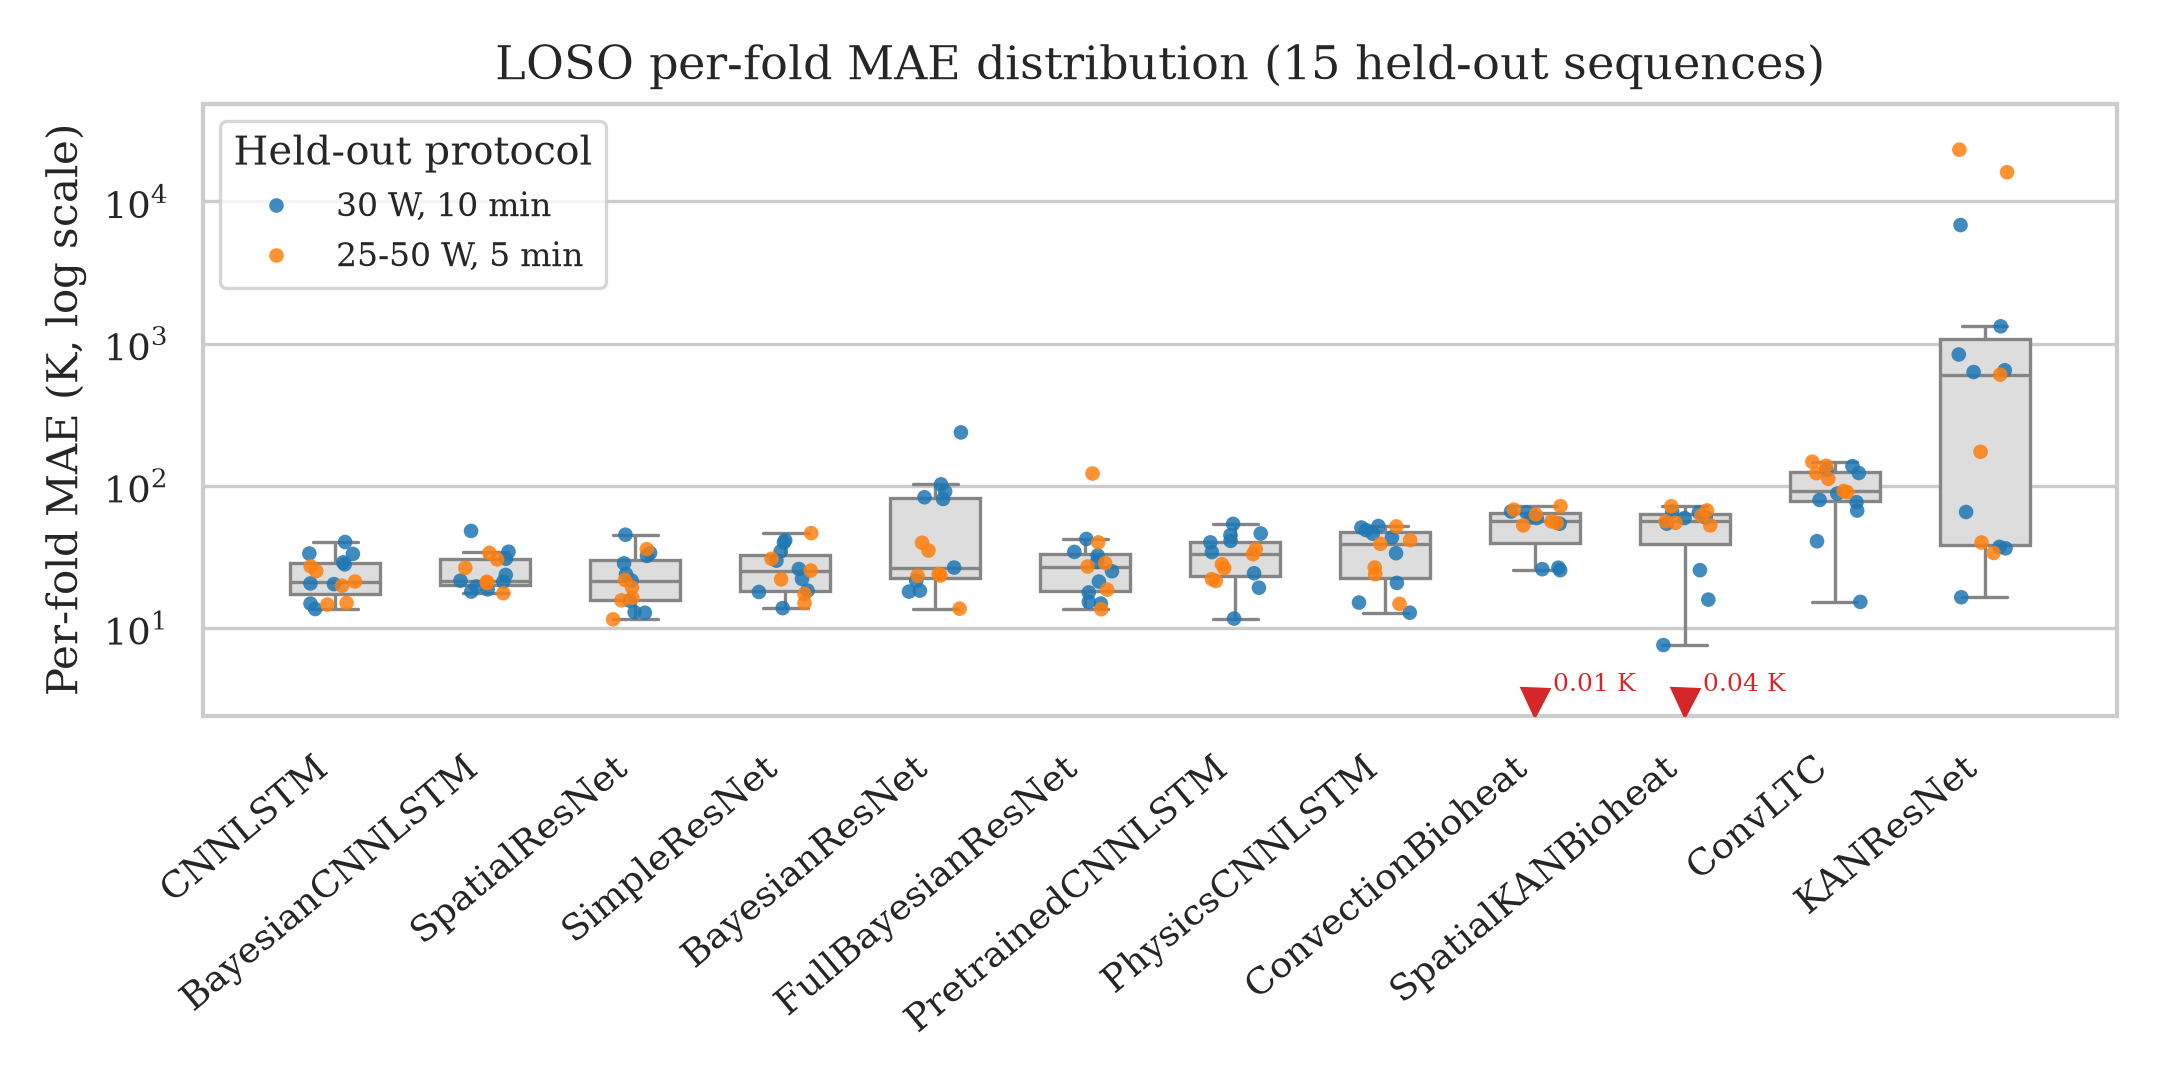
\includegraphics[width=0.85\textwidth]{figures/loso_mae_distribution.png}
\caption{Per-fold LOSO MAE for every model (baseline configuration, log scale), ordered by median. Boxes show the median and interquartile range across the 15 held-out sequences; points are coloured by acquisition protocol. The image-only scalar models (left) overlap almost completely, whereas ConvLTC and KANResNet are shifted upwards by one to three orders of magnitude. The two red markers are the implausibly low fold-001 scores of ConvectionBioheat (0.01\,K) and SpatialKANBioheat (0.04\,K), which are under investigation as a potential evaluation artifact.}
\label{fig:loso_mae_distribution}
\end{figure*}

\begin{figure}[t]
\centering
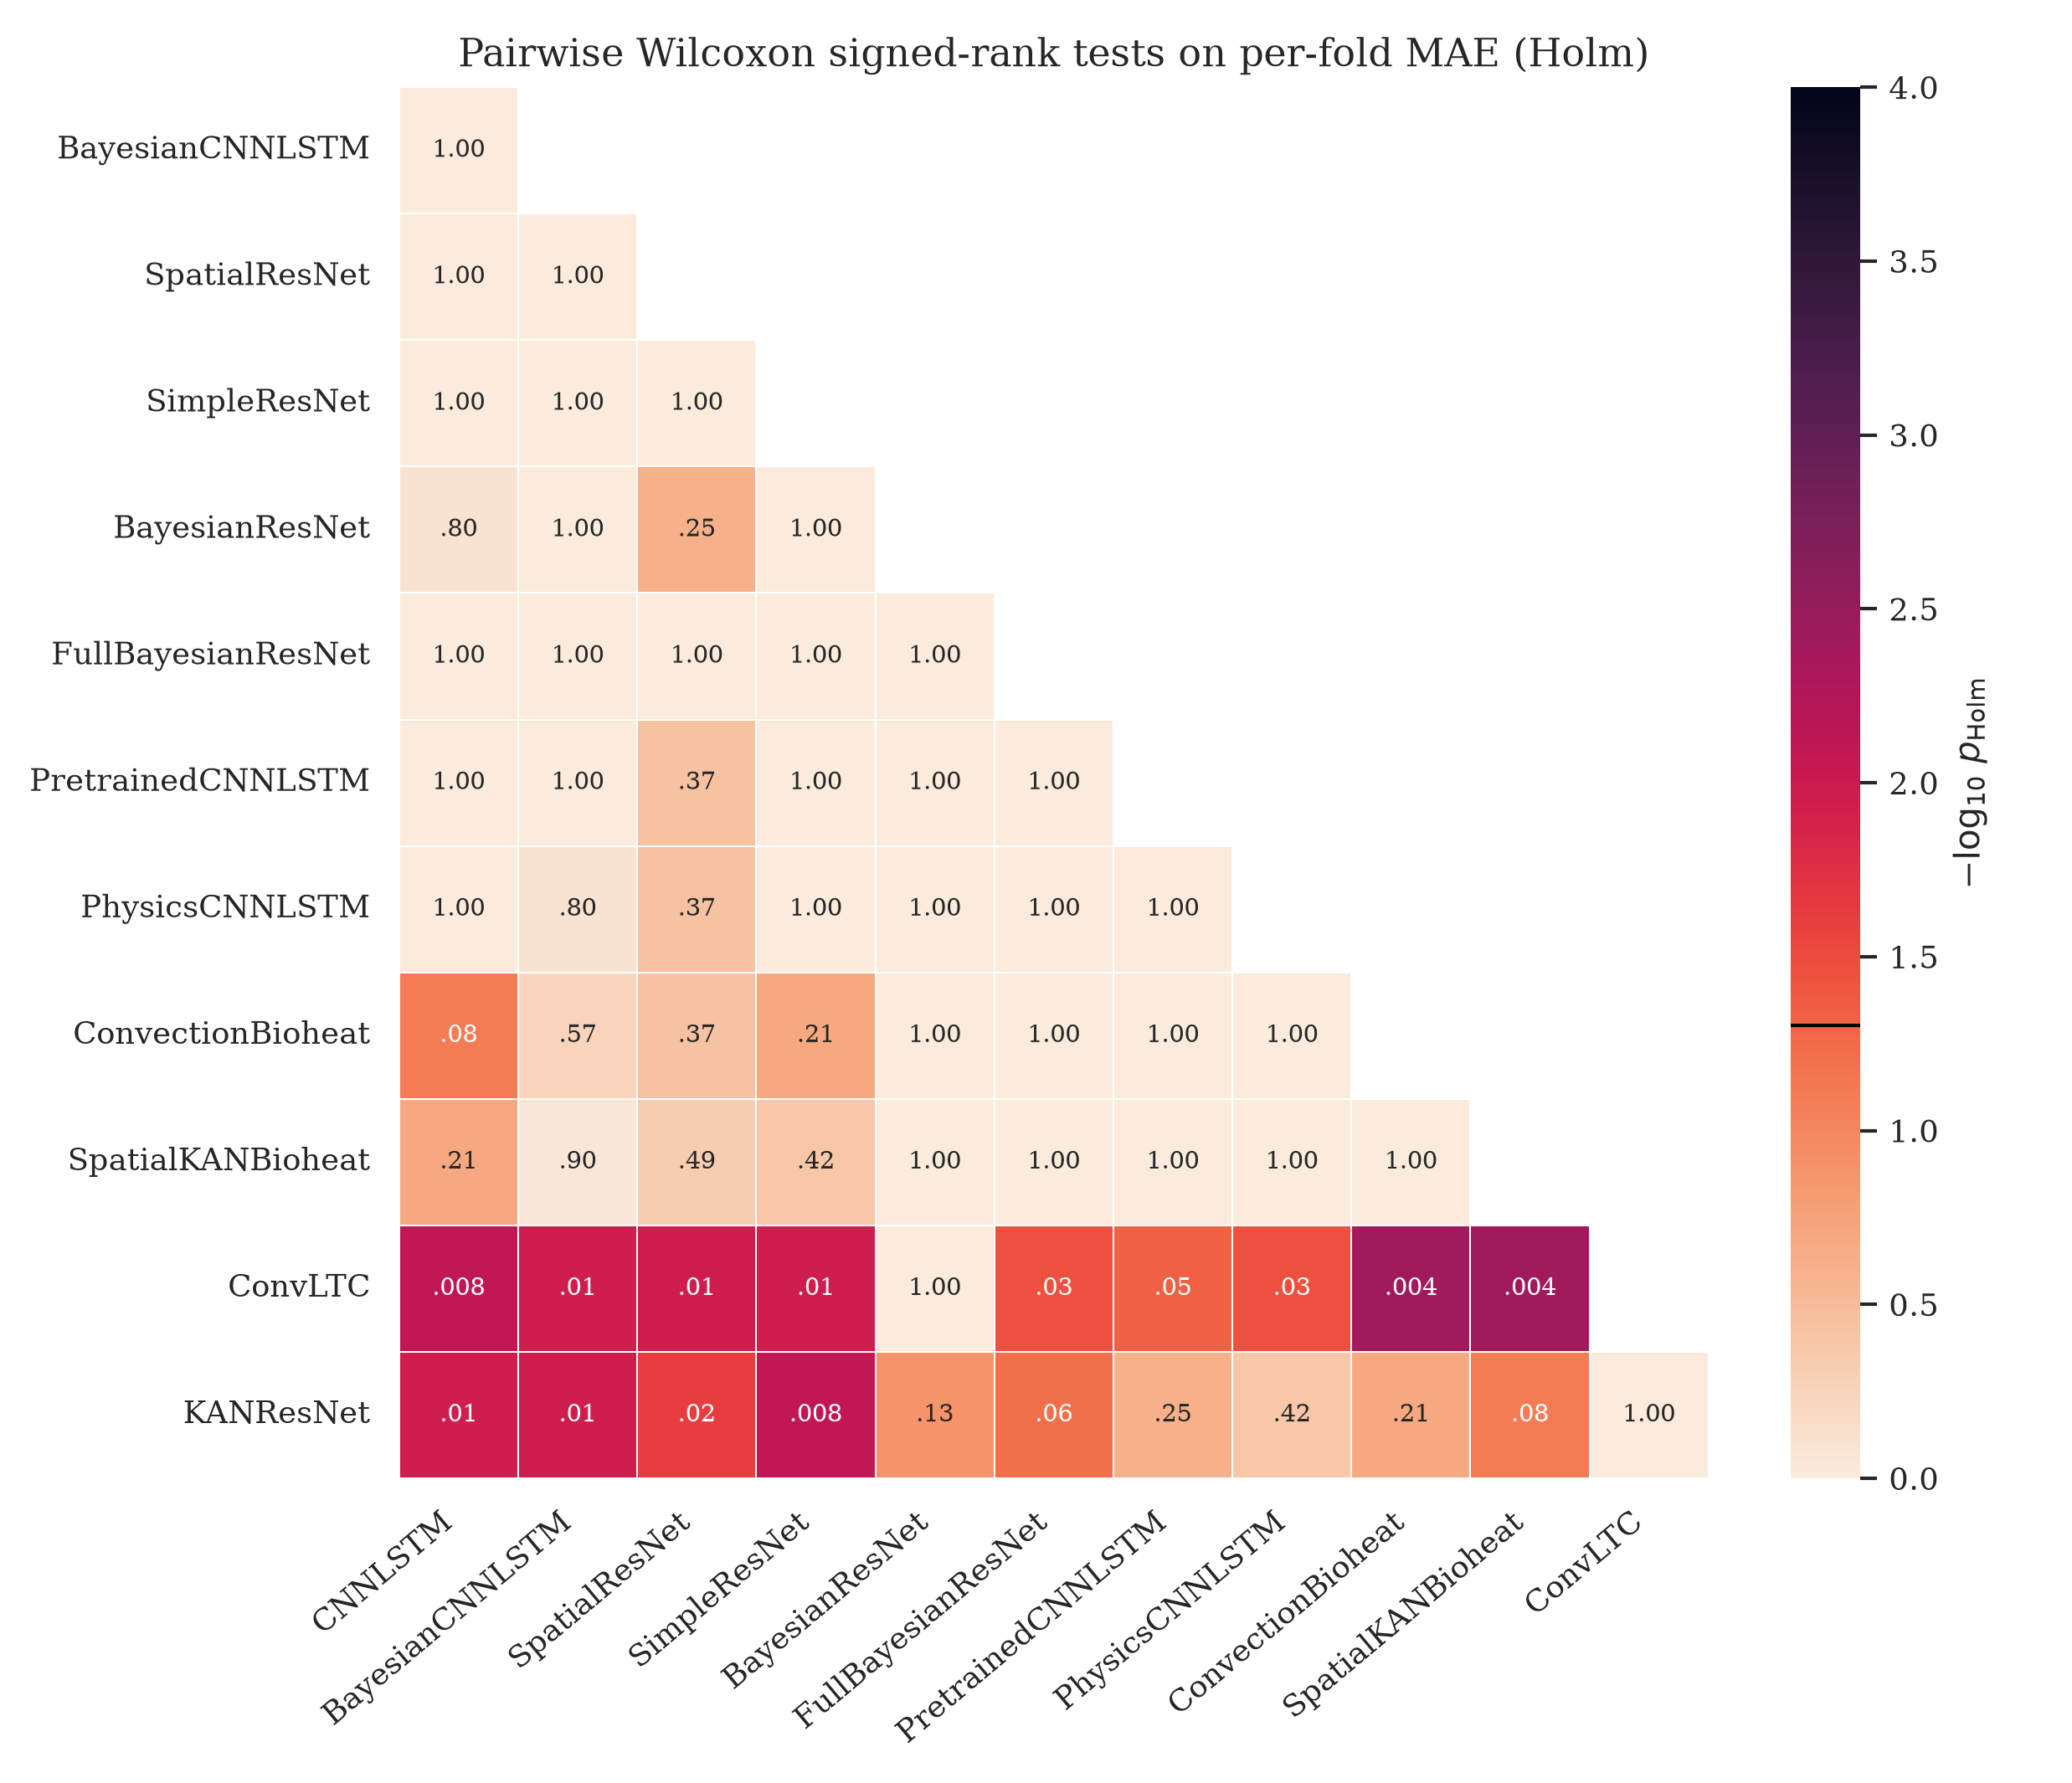
\includegraphics[width=\columnwidth]{figures/loso_wilcoxon_heatmap.png}
\caption{Pairwise two-sided Wilcoxon signed-rank tests on per-fold MAE across all 66 model pairs, Holm-adjusted. Cells show $p_\mathrm{Holm}$; the black line on the colour bar marks $p=0.05$. Only ConvLTC and KANResNet are separable from the leading models after correction.}
\label{fig:loso_wilcoxon_heatmap}
\end{figure}

\begin{figure*}[t]
\centering
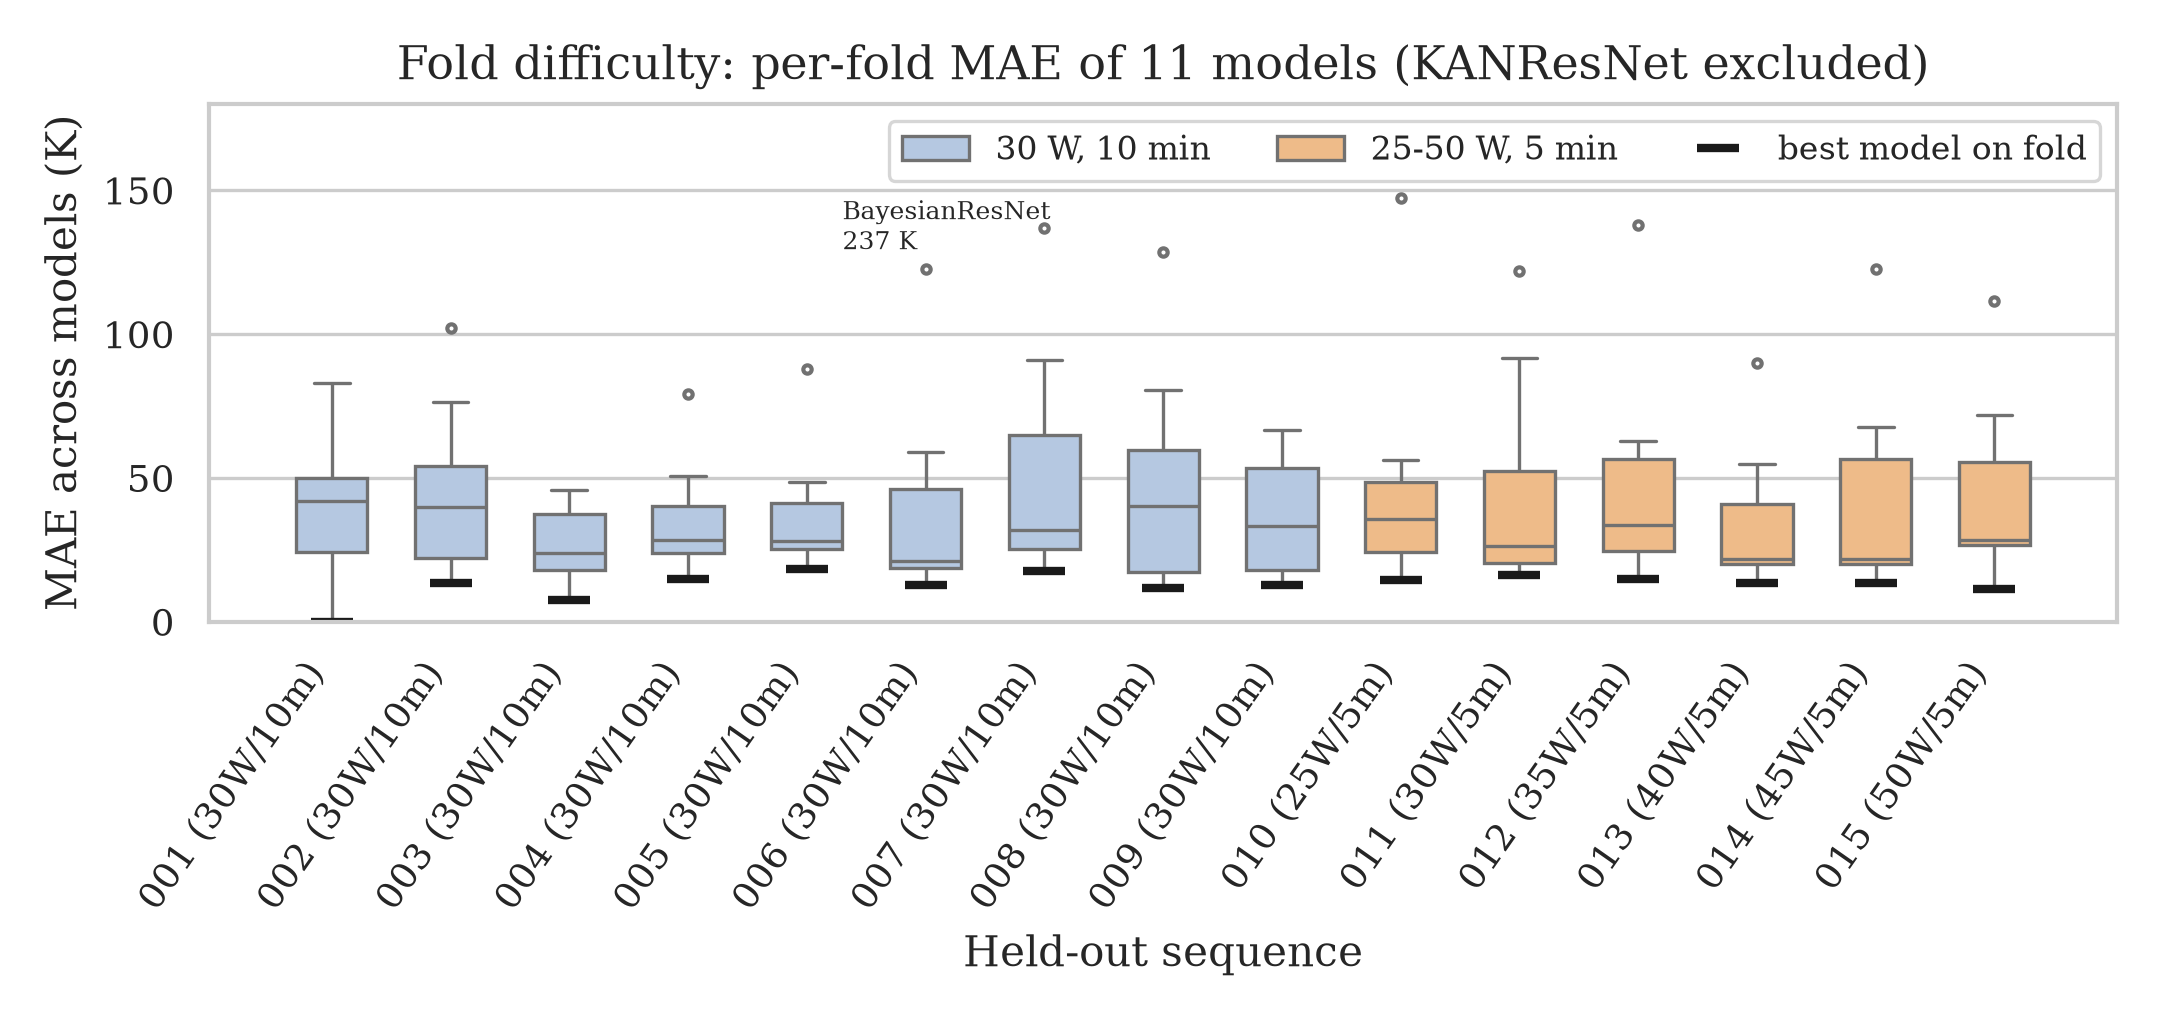
\includegraphics[width=0.85\textwidth]{figures/loso_fold_difficulty.png}
\caption{Fold difficulty: distribution of per-fold MAE across 11 models (KANResNet excluded) for each held-out sequence, labelled by index, ablation power, and duration. Black ticks mark the best model on each fold. The best achievable MAE lies between 7.6 and 18.3\,K on every fold except 001 (see Fig.~\ref{fig:loso_mae_distribution}); one off-scale BayesianResNet fold is annotated.}
\label{fig:loso_fold_difficulty}
\end{figure*}
